\documentclass[11pt,a4paper]{report}
\usepackage[textwidth=37em,vmargin=30mm]{geometry}
\usepackage{calc,xunicode,amsmath,amssymb,paralist,enumitem,tabu,booktabs,datetime2,xeCJK,xeCJKfntef,listings}
\usepackage{tocloft,fancyhdr,tcolorbox,xcolor,graphicx,eso-pic,xltxtra,xelatexemoji}

\newcommand{\envyear}[0]{2025}
\newcommand{\envdatestr}[0]{2025-01-09}
\newcommand{\envfinaldir}[0]{webdb/2025/20250109/final}

\usepackage[hidelinks]{hyperref}
\hypersetup{
    colorlinks=false,
    pdfpagemode=FullScreen,
    pdftitle={Web Digest - \envdatestr}
}

\setlength{\cftbeforechapskip}{10pt}
\renewcommand{\cftchapfont}{\rmfamily\bfseries\large\raggedright}
\setlength{\cftbeforesecskip}{2pt}
\renewcommand{\cftsecfont}{\sffamily\small\raggedright}

\setdefaultleftmargin{2em}{2em}{1em}{1em}{1em}{1em}

\usepackage{xeCJK,xeCJKfntef}
\xeCJKsetup{PunctStyle=plain,RubberPunctSkip=false,CJKglue=\strut\hskip 0pt plus 0.1em minus 0.05em,CJKecglue=\strut\hskip 0.22em plus 0.2em}
\XeTeXlinebreaklocale "zh"
\XeTeXlinebreakskip = 0pt


\setmainfont{Brygada 1918}
\setromanfont{Brygada 1918}
\setsansfont{IBM Plex Sans}
\setmonofont{JetBrains Mono NL}
\setCJKmainfont{Noto Serif CJK SC}
\setCJKromanfont{Noto Serif CJK SC}
\setCJKsansfont{Noto Sans CJK SC}
\setCJKmonofont{Noto Sans CJK SC}

\setlength{\parindent}{0pt}
\setlength{\parskip}{8pt}
\linespread{1.15}

\lstset{
	basicstyle=\ttfamily\footnotesize,
	numbersep=5pt,
	backgroundcolor=\color{black!5},
	showspaces=false,
	showstringspaces=false,
	showtabs=false,
	tabsize=2,
	captionpos=b,
	breaklines=true,
	breakatwhitespace=true,
	breakautoindent=true,
	linewidth=\textwidth
}






\newcommand{\coverpic}[2]{
    % argv: itemurl, authorname
    Cover photo by #2~~(\href{#1}{#1})
}
\newcommand{\makeheader}[0]{
    \begin{titlepage}
        % \newgeometry{hmargin=15mm,tmargin=21mm,bmargin=12mm}
        \begin{center}
            
            \rmfamily\scshape
            \fontspec{BaskervilleF}
            \fontspec{Old Standard}
            \fontsize{59pt}{70pt}\selectfont
            WEB\hfill DIGEST
            
            \vfill
            % \vskip 30pt
            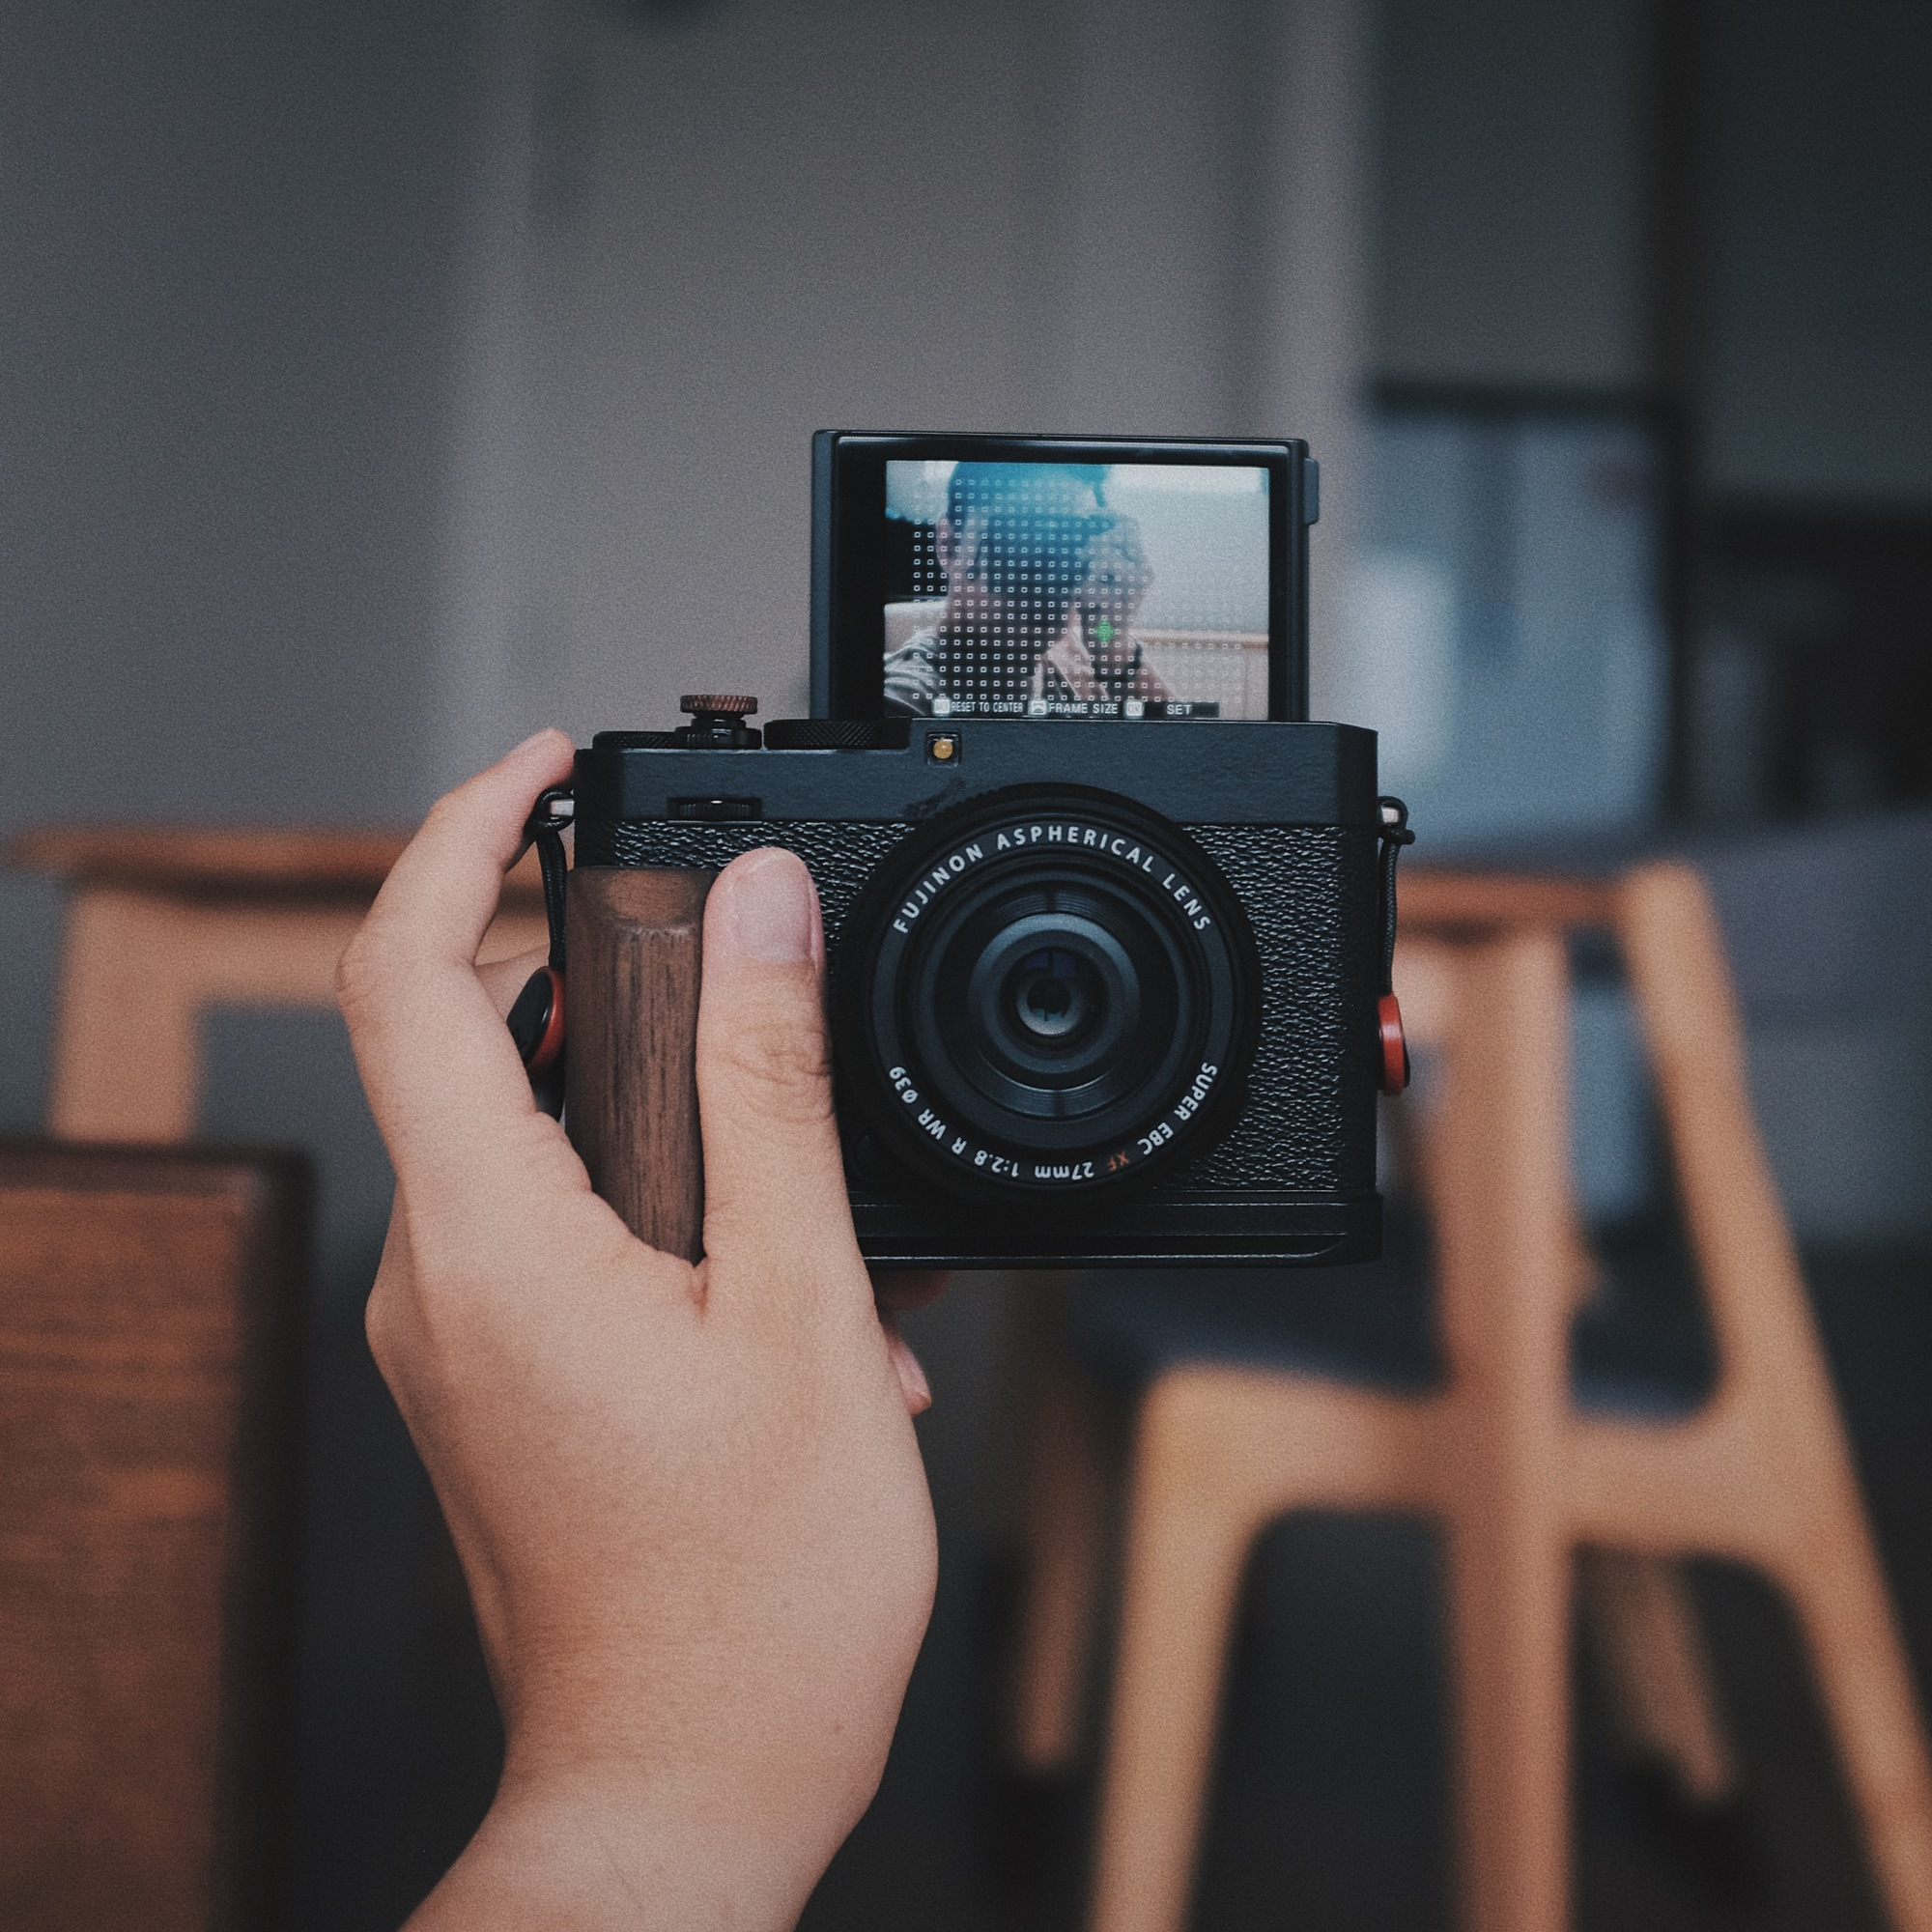
\includegraphics[width=\linewidth]{\envfinaldir/coverpic-prod.jpg}\par
            % \vskip 30pt
            \vfill

            \normalsize\rmfamily\scshape
            \copyright{} The Web Digest Project \hfill\large \envdatestr
        \end{center}
    \end{titlepage}
    % \restoregeometry
}
\newcommand{\simplehref}[1]{%
    \textcolor{blue!80!green}{\href{#1}{#1}}%
}
\renewcommand{\contentsname}{\center\Huge\sffamily\bfseries Contents\par\vskip 20pt}
\newcounter{ipartcounter}
\setcounter{ipartcounter}{0}
\newcommand{\ipart}[1]{
    % \vskip 20pt
    \clearpage
    \stepcounter{ipartcounter}
    \phantomsection
    \addcontentsline{toc}{chapter}{#1}
    % \begin{center}
    %     \Huge
    %     \sffamily\bfseries
    %     #1
    % \end{center}
    % \vskip 20pt plus 7pt
}
\newcounter{ichaptercounter}
\setcounter{ichaptercounter}{0}
\newcommand{\ichapter}[1]{
    % \vskip 20pt
    \clearpage
    \stepcounter{ichaptercounter}
    \phantomsection
    \addcontentsline{toc}{section}{\numberline{\arabic{ichaptercounter}}#1}
    \begin{center}
        \Huge
        \sffamily\bfseries
        #1
    \end{center}
    \vskip 20pt plus 7pt
}
\newcommand{\entrytitlefont}[1]{\subsection*{\raggedright\Large\sffamily\bfseries#1}}
\newcommand{\entryitemGeneric}[2]{
    % argv: title, url
    \parbox{\linewidth}{
        \entrytitlefont{#1}\par\vskip 5pt
        \footnotesize\ttfamily\mdseries
        \simplehref{#2}
    }\vskip 11pt plus 11pt minus 1pt
}
\newcommand{\entryitemGithub}[3]{
    % argv: title, url, desc
    \parbox{\linewidth}{
        \entrytitlefont{#1}\par\vskip 5pt
        \footnotesize\ttfamily\mdseries
        \simplehref{#2}\par\vskip 5pt
        \small\rmfamily\mdseries#3
    }\vskip 11pt plus 11pt minus 1pt
}
\newcommand{\entryitemAp}[3]{
    % argv: title, url, desc
    \parbox{\linewidth}{
        \entrytitlefont{#1}\par\vskip 5pt
        \footnotesize\ttfamily\mdseries
        \simplehref{#2}\par\vskip 5pt
        \small\rmfamily\mdseries#3
    }\vskip 11pt plus 11pt minus 1pt
}
\newcommand{\entryitemHackernews}[3]{
    % argv: title, hnurl, rawurl
    % \parbox{\linewidth}{
    %     \entrytitlefont{#1}\par\vskip 5pt
    %     \footnotesize\ttfamily\mdseries
    %     \simplehref{#3}\par
    %     \textcolor{black!50}{\href{#2}{#2}}
    % }\vskip 11pt plus 11pt minus 1pt
    \begin{minipage}{\linewidth}
            \entrytitlefont{#1}\par\vskip 5pt
            \footnotesize\ttfamily\mdseries
            \simplehref{#3}\par
            \textcolor{black!50}{\href{#2}{#2}}
    \end{minipage}\par\vskip 11pt plus 11pt minus 1pt
}







\begin{document}

\makeheader

\tableofcontents\clearpage




\ipart{Developers}
\ichapter{Hacker News}
\entryitemTwoLinks{LA wildfires force thousands to evacuate, NASA JPL closed}{https://news.ycombinator.com/item?id=42638735}{https://www.theregister.com/2025/01/08/los\_angeles\_fires\_jpl/}

\entryitemTwoLinks{I had to take down my course-swapping site or be expelled}{https://news.ycombinator.com/item?id=42638626}{https://www.linkedin.com/posts/jdkaim\_github-jdkaimhuskyswap-huskyswap-project-activity-7282609173316415488-1jdb}

\entryitemTwoLinks{Facebook is removing stories about pornographic ads}{https://news.ycombinator.com/item?id=42637267}{https://www.404media.co/facebook-is-censoring-404-media-stories-about-facebooks-censorship/}

\entryitemTwoLinks{NeuralSVG: An Implicit Representation for Text-to-Vector Generation}{https://news.ycombinator.com/item?id=42636873}{https://sagipolaczek.github.io/NeuralSVG/}

\entryitemTwoLinks{Bringing SerenityOS to real hardware, one driver at a time}{https://news.ycombinator.com/item?id=42636086}{https://sdomi.pl/weblog/23-serenityos-realhw/}

\entryitemTwoLinks{Show HN: Atlas of Space}{https://news.ycombinator.com/item?id=42634787}{https://atlasof.space/}

\entryitemTwoLinks{Fidget}{https://news.ycombinator.com/item?id=42634624}{https://www.mattkeeter.com/projects/fidget/}

\entryitemTwoLinks{Robotics 101 at UMich: Applied numerical linear algebra as intro linear algebra}{https://news.ycombinator.com/item?id=42633805}{https://robotics.umich.edu/academics/courses/course-offerings/rob101-fall-2020/}

\entryitemTwoLinks{Cracking a 512-bit DKIM key for less than \$8 in the cloud}{https://news.ycombinator.com/item?id=42633501}{https://dmarcchecker.app/articles/crack-512-bit-dkim-rsa-key}

\entryitemTwoLinks{Bye-bye Windows gaming? SteamOS officially expands past the Steam Deck}{https://news.ycombinator.com/item?id=42633269}{https://arstechnica.com/gaming/2025/01/bye-bye-windows-gaming-steamos-officially-expands-past-the-steam-deck/}

\entryitemTwoLinks{The Comet is a handheld Linux computer that brings extensibility}{https://news.ycombinator.com/item?id=42632865}{https://mecha.so/comet}

\entryitemTwoLinks{The Aging Programmer}{https://news.ycombinator.com/item?id=42632772}{https://www.youtube.com/watch?v=mVWQQeSOD0M}

\entryitemTwoLinks{Operating System in 1,000 Lines – Intro}{https://news.ycombinator.com/item?id=42631873}{https://operating-system-in-1000-lines.vercel.app/en}

\entryitemTwoLinks{Gate-level simulation of ASIC in browser}{https://news.ycombinator.com/item?id=42631629}{https://znah.net/tt09/}

\entryitemTwoLinks{Annual 'winners' for most egregious US healthcare profiteering announced}{https://news.ycombinator.com/item?id=42630030}{https://www.theguardian.com/us-news/2025/jan/07/annual-awards-healthcare-profiteering}

\entryitemTwoLinks{Oracle Will Not Voluntarily Withdraw JavaScript Trademark}{https://news.ycombinator.com/item?id=42629256}{https://twitter.com/deno\_land/status/1876728474666217739}

\entryitemTwoLinks{A day in the life of a prolific voice phishing crew}{https://news.ycombinator.com/item?id=42629163}{https://krebsonsecurity.com/2025/01/a-day-in-the-life-of-a-prolific-voice-phishing-crew/}

\entryitemTwoLinks{Automated accessibility testing at Slack}{https://news.ycombinator.com/item?id=42628934}{https://slack.engineering/automated-accessibility-testing-at-slack/}

\entryitemTwoLinks{Servo Revival: 2023-2024}{https://news.ycombinator.com/item?id=42628414}{https://blogs.igalia.com/mrego/servo-revival-2023-2024/}

\entryitemTwoLinks{Laid off for the first time in my career, and twice in one year}{https://news.ycombinator.com/item?id=42627567}{https://dillonshook.com/laid-off/}\ichapter{Phoronix}
\entryitemGeneric{\hskip 0pt{}Intel's Clang Code Begins Landing For OpenMP Offloading To SPIR-V For GPU Execution}{https://www.phoronix.com/news/Intel-Clang-OpenMP-To-SPIR-V}

\entryitemGeneric{\hskip 0pt{}Linux 6.14 Preps UHBR For Intel Panther Lake, Lower Alchemist GPU Power Use With Whitelisted CPUs}{https://www.phoronix.com/news/Linux-6.14-Intel-UHBR-TB}

\entryitemGeneric{\hskip 0pt{}AMD Linux GPU Driver Preps OEM i2c Bus Support Used For RGB Control \& More}{https://www.phoronix.com/news/AMDGPU-More-i2c-Bus}

\entryitemGeneric{\hskip 0pt{}Intel Preps Nice NPU Driver Improvements For Linux 6.14}{https://www.phoronix.com/news/Intel-NPU-Linux-6.14-IVPU}

\entryitemGeneric{\hskip 0pt{}FEX 2501 Brings JIT Performance Improvements, Changes Needed For Denuvo Support}{https://www.phoronix.com/news/FEX-Emulator-2501}

\entryitemGeneric{\hskip 0pt{}KDE Plasma 6.3 To Offer Better Night Light Mode On HDR Displays}{https://www.phoronix.com/news/KDE-Plasma-6.3-Night-Light-HDR}

\entryitemGeneric{\hskip 0pt{}Open3D v0.19 Brings Cross-Platform GPU Support Via SYCL}{https://www.phoronix.com/news/Open3D-v0.19-Released}

\entryitemGeneric{\hskip 0pt{}Arch Linux User Repository Requires Packages To Support x86\_64: No ARM-Only Software}{https://www.phoronix.com/news/Arch-Linux-AUR-Requires-x86\_64}

\entryitemGeneric{\hskip 0pt{}Cross-Vendor Mesh Shading Being Worked On For OpenGL}{https://www.phoronix.com/news/OpenGL-GL\_EXT\_mesh\_shader}


\ipart{Developers~~~~(zh-Hans)}
\ichapter{Solidot}
\entryitemGeneric{\hskip 0pt{}Akamai 将终止在中国的 CDN 服务}{https://www.solidot.org/story?sid=80275}

\entryitemGeneric{\hskip 0pt{}泰国禁止进口塑料垃圾}{https://www.solidot.org/story?sid=80274}

\entryitemGeneric{\hskip 0pt{}Meta 取消事实核查}{https://www.solidot.org/story?sid=80273}

\entryitemGeneric{\hskip 0pt{}委内瑞拉限制了 TikTok 的访问}{https://www.solidot.org/story?sid=80272}

\entryitemGeneric{\hskip 0pt{}睡眠不足能减弱排除不愉快记忆的能力}{https://www.solidot.org/story?sid=80271}

\entryitemGeneric{\hskip 0pt{}Cyber​​truck 爆炸案嫌疑人使用 ChatGPT 出谋划策}{https://www.solidot.org/story?sid=80270}

\entryitemGeneric{\hskip 0pt{}个人计算机 Altair 8800 发布 50 周年}{https://www.solidot.org/story?sid=80269}

\entryitemGeneric{\hskip 0pt{}俄罗斯 ISP Nodex 遭乌克兰网络攻击导致全面断网}{https://www.solidot.org/story?sid=80268}

\entryitemGeneric{\hskip 0pt{}联想与 Valve 合作推出首款预装 SteamOS 的第三方掌机}{https://www.solidot.org/story?sid=80267}

\entryitemGeneric{\hskip 0pt{}盖蒂和 Shutterstock 宣布合并}{https://www.solidot.org/story?sid=80266}

\entryitemGeneric{\hskip 0pt{}中科院计划今年推出高性能 RISC-V 处理器香山}{https://www.solidot.org/story?sid=80265}

\entryitemGeneric{\hskip 0pt{}西藏定日地震造成逾百人死亡}{https://www.solidot.org/story?sid=80264}

\entryitemGeneric{\hskip 0pt{}开发者创造出基于噩梦难度 Doom 的可玩 CAPTCHA }{https://www.solidot.org/story?sid=80263}

\entryitemGeneric{\hskip 0pt{}安全公司建议不支持 Windows 11 的电脑安装 Linux}{https://www.solidot.org/story?sid=80262}

\entryitemGeneric{\hskip 0pt{}微软呼吁 Windows 10 用户换电脑}{https://www.solidot.org/story?sid=80261}

\entryitemGeneric{\hskip 0pt{}罗马帝国大规模使用铅降低了欧洲居民的智商}{https://www.solidot.org/story?sid=80260}

\entryitemGeneric{\hskip 0pt{}同样的食物为什么对每个人的影响不同}{https://www.solidot.org/story?sid=80259}

\entryitemGeneric{\hskip 0pt{}日本 2024 年平均气温创新纪录}{https://www.solidot.org/story?sid=80258}

\entryitemGeneric{\hskip 0pt{}1/10 新2型糖尿病可能是含糖饮料引起的}{https://www.solidot.org/story?sid=80257}

\entryitemGeneric{\hskip 0pt{}AMD 宣布第二代掌机芯片}{https://www.solidot.org/story?sid=80256}\ichapter{V2EX}
\entryitemGeneric{\hskip 0pt{}[酷工作] 腾讯游戏内推}{https://www.v2ex.com/t/1103734}

\entryitemGeneric{\hskip 0pt{}[分享发现] 移动套餐内语音比套餐外贵}{https://www.v2ex.com/t/1103733}

\entryitemGeneric{\hskip 0pt{}[VPS] 速报:搬瓦工将在未来 48 小时内给主机配上 IPv6}{https://www.v2ex.com/t/1103732}

\entryitemGeneric{\hskip 0pt{}[阅读] 2024 十二月读美国史 小说…… 4 本}{https://www.v2ex.com/t/1103730}

\entryitemGeneric{\hskip 0pt{}[问与答] 求推荐安卓看 epub 的软件}{https://www.v2ex.com/t/1103728}

\entryitemGeneric{\hskip 0pt{}[问与答] 目前国内,甚至全世界,有人车家全生态产品的,是不是只有小米?}{https://www.v2ex.com/t/1103727}

\entryitemGeneric{\hskip 0pt{}[程序员] 关于 XHTTP 协议}{https://www.v2ex.com/t/1103724}

\entryitemGeneric{\hskip 0pt{}[Kubernetes] k8s 新人求助帖}{https://www.v2ex.com/t/1103721}

\entryitemGeneric{\hskip 0pt{}[分享创造] [开源分享|抛砖引玉] Tabless 一款可以让你在新标签中摸鱼划水的浏览器插件}{https://www.v2ex.com/t/1103720}

\entryitemGeneric{\hskip 0pt{}[生活] paypal 自动付款被收取货币兑换手续费}{https://www.v2ex.com/t/1103719}

\entryitemGeneric{\hskip 0pt{}[Telegram] tg 那些热门机器人是如何做到快速响应的?}{https://www.v2ex.com/t/1103718}

\entryitemGeneric{\hskip 0pt{}[分享发现] 自己上架应用真不容易}{https://www.v2ex.com/t/1103717}

\entryitemGeneric{\hskip 0pt{}[Flutter] flutter 启动 ios 项目失败 n 次,求大神帮忙}{https://www.v2ex.com/t/1103716}

\entryitemGeneric{\hskip 0pt{}[OpenAI] 有没有人用 firstrade 的 visa debit card 给 openai 充值?}{https://www.v2ex.com/t/1103714}

\entryitemGeneric{\hskip 0pt{}[问与答] 各位技术大佬,现场大屏通过微信扫码进行抽奖 有没有现成的?}{https://www.v2ex.com/t/1103713}

\entryitemGeneric{\hskip 0pt{}[推广] 送码,送码,永久兑换码,需要的评论留言}{https://www.v2ex.com/t/1103712}

\entryitemGeneric{\hskip 0pt{}[酷工作] [全职远程]英国伦敦二次元手游公司直招 unity 开发工程师}{https://www.v2ex.com/t/1103710}

\entryitemGeneric{\hskip 0pt{}[问与答] 假如你是站长, 你该怎么回?}{https://www.v2ex.com/t/1103708}

\entryitemGeneric{\hskip 0pt{}[职场话题] 年底是跳槽的时候么}{https://www.v2ex.com/t/1103706}

\entryitemGeneric{\hskip 0pt{}[Apple] 买外版苹果,账号也得转外区啊}{https://www.v2ex.com/t/1103704}

\entryitemGeneric{\hskip 0pt{}[问与答] 去日本玩带 5090 过海关用交税吗?}{https://www.v2ex.com/t/1103701}

\entryitemGeneric{\hskip 0pt{}[酷工作] 远程岗位内推,简历直推 HR}{https://www.v2ex.com/t/1103699}

\entryitemGeneric{\hskip 0pt{}[硬件] AMD 显卡 / APU 睡眠结束后显示器黑屏问题的解决经历}{https://www.v2ex.com/t/1103697}

\entryitemGeneric{\hskip 0pt{}[推广] 自家茶山产安吉白茶 24 年新茶(接受 25 年新茶预定)}{https://www.v2ex.com/t/1103692}

\entryitemGeneric{\hskip 0pt{}[程序员] 游戏开发中经常需要使用低多面体(Low Poly)、为游戏优化的模型,是否意味着现在显卡算力还远没有达到能够实时渲染电影级画面的水平?}{https://www.v2ex.com/t/1103689}

\entryitemGeneric{\hskip 0pt{}[上海] 上海个人转租——3 号线张华浜地铁站 杨浦、虹口上班方便}{https://www.v2ex.com/t/1103688}

\entryitemGeneric{\hskip 0pt{}[Apple] AppStore 貌似更改了跨账号内购的规定}{https://www.v2ex.com/t/1103687}

\entryitemGeneric{\hskip 0pt{}[宽带症候群] 10G / 2.5G 的个人宽带有什么用}{https://www.v2ex.com/t/1103684}

\entryitemGeneric{\hskip 0pt{}[Java] 最近公司在搞防重,有很多账务类相关的}{https://www.v2ex.com/t/1103682}

\entryitemGeneric{\hskip 0pt{}[Steam] steam deck oled 玩小小梦魇 2 加强版一开光追就卡,如何解决?}{https://www.v2ex.com/t/1103681}

\entryitemGeneric{\hskip 0pt{}[Apple] iOS18.3beta2 升级后国产 App 挂了一大半}{https://www.v2ex.com/t/1103677}

\entryitemGeneric{\hskip 0pt{}[问与答] 关于小狼毫输入法的问题,有什么快捷键可以删除上一次打的词语呢?}{https://www.v2ex.com/t/1103676}

\entryitemGeneric{\hskip 0pt{}[程序员] 在线体验 DeepSeek 编写代码的能力}{https://www.v2ex.com/t/1103672}

\entryitemGeneric{\hskip 0pt{}[职场话题] 程序员到 35 岁可以考虑 gap 吗?}{https://www.v2ex.com/t/1103666}

\entryitemGeneric{\hskip 0pt{}[问与答] 淘宝上面帮别人代付软件是什么渠道?比如我看到淘宝卖 Cursor 一个月才几十块钱。}{https://www.v2ex.com/t/1103656}

\entryitemGeneric{\hskip 0pt{}[设计] 室内设计师们都用什么软件?效果图,安装图/施工图,🙏}{https://www.v2ex.com/t/1103653}

\entryitemGeneric{\hskip 0pt{}[北京] 朝阳区 14 号线东风北桥旁卧室带独卫 转租}{https://www.v2ex.com/t/1103651}

\entryitemGeneric{\hskip 0pt{}[RSS] feedly 好像炸了}{https://www.v2ex.com/t/1103647}

\entryitemGeneric{\hskip 0pt{}[分享创造] 做了个 Jujutsu Infinite 新闻\&攻略站,有玩这个游戏的么?进来给些意见建议}{https://www.v2ex.com/t/1103644}

\entryitemGeneric{\hskip 0pt{}[问与答] 人肉搜索和开盒的技术原理是什么?}{https://www.v2ex.com/t/1103643}

\entryitemGeneric{\hskip 0pt{}[问与答] 穿羽毛球服去健身房会不会有点怪?}{https://www.v2ex.com/t/1103642}

\entryitemGeneric{\hskip 0pt{}[问与答] 有没有横向评测的工具或者网站可以快速根据关键词生成关系网?}{https://www.v2ex.com/t/1103640}

\entryitemGeneric{\hskip 0pt{}[程序员] cursor @web 能力咋不行}{https://www.v2ex.com/t/1103639}

\entryitemGeneric{\hskip 0pt{}[分享发现] 是我手机有问题么,刚刚打开美团/饿了么都给我定位到江西九江去了}{https://www.v2ex.com/t/1103638}

\entryitemGeneric{\hskip 0pt{}[分享发现] 致态 ti600 1TB 的奇怪问题}{https://www.v2ex.com/t/1103637}

\entryitemGeneric{\hskip 0pt{}[分享创造] 分享一下我用 AI 从 0 到 1 开发 App 的经验, the good, the bad, the ugly.}{https://www.v2ex.com/t/1103636}

\entryitemGeneric{\hskip 0pt{}[Google] 请问, 有没有大佬可以帮忙激活一下 googke FI ,有偿,谢谢}{https://www.v2ex.com/t/1103635}

\entryitemGeneric{\hskip 0pt{}[问与答] pc 端的 qq 和微信 wechat 如何修改默认字体}{https://www.v2ex.com/t/1103634}

\entryitemGeneric{\hskip 0pt{}[汽车] 25 年汽车补贴政策出来了,家里的老面包正好满足,想给老爸换个车,平时市区周边活动,基本不出远门,大家有什么推荐吗?}{https://www.v2ex.com/t/1103633}

\entryitemGeneric{\hskip 0pt{}[分享发现] rising star js 昨天更新 2024 年内容了,感觉很多都没用过啊}{https://www.v2ex.com/t/1103632}


\ipart{Generic News}
\ichapter{AP News}
\entryitemWithDescription{\hskip 0pt{}`Wicked' tops SAG Awards nominations as many big names are snubbed}{https://apnews.com/article/8936e2b217c60555067828c8812ec706}{}

\entryitemWithDescription{\hskip 0pt{}Outdoor hockey is coming to Florida. The NHL will have games in Miami and Tampa next season}{https://apnews.com/article/a5ffa36c8036334bb39c340488456657}{}

\entryitemWithDescription{\hskip 0pt{}Egypt unveils ancient rock-cut tombs and burial shafts in Luxor}{https://apnews.com/article/ea6f55316dd0abdfb6a4c34f97838962}{}

\entryitemWithDescription{\hskip 0pt{}Man accused of stockpiling 150 homemade bombs must stay in jail until trial, judge rules}{https://apnews.com/article/eac9b300d04f4f1760e2ed226b14f61f}{}

\entryitemWithDescription{\hskip 0pt{}Former Baltimore Orioles left-hander Brian Matusz dies at 37, no cause of death announced}{https://apnews.com/article/2a045729d0906ea20d032b965e620491}{}

\entryitemWithDescription{\hskip 0pt{}JetBlue passenger suddenly opens exit door as flight is taxiing for takeoff at Boston airport}{https://apnews.com/article/4884322a676055d0ab5d858e7d33b4b1}{}

\entryitemWithDescription{\hskip 0pt{}Expected guilty plea for man in `Wizard of Oz' ruby slippers case postponed due to hospitalization}{https://apnews.com/article/89b213b57a7a9fdbed4240a7ffc5717e}{}

\entryitemWithDescription{\hskip 0pt{}Peter Yarrow of folk-music trio Peter, Paul and Mary dies at 86}{https://apnews.com/article/767c223e40c243199b0d0875e29a5efc}{}

\entryitemWithDescription{\hskip 0pt{}NASA proposes cheaper and quicker way to get Mars rocks and soil to Earth}{https://apnews.com/article/6b6028cd2866f41f39864717f70e979d}{}

\entryitemWithDescription{\hskip 0pt{}Donald Trump Jr. arrives in Greenland with a message from his dad: `We're going to treat you well'}{https://apnews.com/article/56bc01f1d3431c035b22ad6564579938}{}

\entryitemWithDescription{\hskip 0pt{}Trump says he will change the name of the Gulf of Mexico. Can he do that?}{https://apnews.com/article/bc438f4feca1234475a1adef99344da7}{}

\entryitemWithDescription{\hskip 0pt{}San Diego State University frat members charged after pledge set on fire at party, prosecutors say}{https://apnews.com/article/140f97800826c4e08f586f37f60c778c}{}

\entryitemWithDescription{\hskip 0pt{}2 sons of Mexican cartel leader `El Chapo' are in plea negotiations with US, attorneys say}{https://apnews.com/article/da8c7f5df283255c389a527c26193b63}{}\ichapter{Reuters}
\entryitemWithDescription{\hskip 0pt{}Biden to meet virtually with Japanese and Philippine leaders, White House says}{https://www.reuters.com/world/biden-meet-virtually-with-japanese-philippine-leaders-white-house-says-2025-01-08/}{U.S. President Joe Biden will host a virtual meeting with leaders from Japan and the Philippines during his trip to Rome this week, the White House said on...}

\entryitemWithDescription{\hskip 0pt{}US to announce new weapons package for Ukraine as defense leaders prepare to meet in Germany}{https://www.reuters.com/world/us-announce-new-weapons-package-ukraine-defense-leaders-prepare-meet-germany-2025-01-08/}{The U.S. is expected to announce \$500 million in military aid for Ukraine on Thursday at a final gathering of President Joe Biden\textquotesingle s weapons pledging conferences, meetings Kyiv says have been critical to its defense...}

\entryitemWithDescription{\hskip 0pt{}Greenland greets Trump interest with MAGA caps but mixed feelings}{https://www.reuters.com/world/europe/greenland-greets-trump-interest-with-maga-caps-mixed-feelings-2025-01-08/}{The renewed interest by U.S. President-elect Donald Trump in Greenland has been greeted enthusiastically by some Greenlanders, although others say the semi-autonomous territory of Denmark is not for...}

\entryitemWithDescription{\hskip 0pt{}NATO membership only credible security guarantee for Ukraine, Finnish foreign minister says}{https://www.reuters.com/world/europe/nato-membership-only-credible-security-guarantee-ukraine-finnish-foreign-2025-01-08/}{Membership in NATO is the only credible long-term security guarantee Ukraine can receive against future Russian aggression, Finland\textquotesingle s top diplomat said on...}

\entryitemWithDescription{\hskip 0pt{}Gunfire heard near the presidency of Chad's capital, military vehicles seen}{https://www.reuters.com/world/africa/gunshots-heard-near-presidency-chad-capital-ndjamena-residents-afp-say-2025-01-08/}{Bursts of gunfire rang out near the presidency in Chad\textquotesingle s capital N\textquotesingle Djamena on Wednesday evening, two residents in the area told...}

\entryitemWithDescription{\hskip 0pt{}US, French troops could secure Syria's northern border, Syrian Kurdish official says}{https://www.reuters.com/world/us-french-troops-could-secure-syrias-northern-border-syrian-kurdish-official-2025-01-08/}{The talks are a part of efforts to defuse conflict between Turkey and Western-backed Kurdish Syrian...}

\entryitemWithDescription{\hskip 0pt{}Zelenskiy, Moldova's Sandu discuss Ukrainian coal to ease Transdniestria energy crisis}{https://www.reuters.com/world/europe/ukraines-zelenskiy-moldovas-sandu-discuss-ukrainian-coal-ease-transdniestria-2025-01-08/}{Ukrainian President Volodymyr Zelenskiy and Moldovan President Maia Sandu on Wednesday discussed using Ukrainian coal to ease the energy crisis which has subjected Moldova\textquotesingle s separatist Transdniestria region to blackouts...}

\entryitemWithDescription{\hskip 0pt{}PM Fico says he secured gas supply for Slovakia in talks with Putin}{https://www.reuters.com/business/energy/pm-fico-says-he-secured-gas-supply-slovakia-talks-with-putin-2025-01-08/}{Prime Minister Robert Fico said on Wednesday he had secured Slovakia\textquotesingle s gas supply during a visit to meet Russian President Vladimir Putin in Moscow last month, just before Ukraine halted the transit of gas from Russia at...}

\entryitemWithDescription{\hskip 0pt{}Romania to rerun presidential election on May 4, ruling coalition party says}{https://www.reuters.com/world/europe/romania-rerun-presidential-election-may-4-ruling-coalition-party-says-2025-01-08/}{Romania\textquotesingle s ruling coalition agreed on Wednesday to rerun a two-round presidential election on May 4 and May 18 and stuck to an original plan to endorse a single candidate, the Liberal Party, one of the three coalition...}

\entryitemWithDescription{\hskip 0pt{}Congo rebels muddy minerals market with illegal Rwanda exports, says UN report}{https://www.reuters.com/world/africa/congo-rebels-muddy-minerals-market-with-illegal-rwanda-exports-says-un-report-2025-01-08/}{Rebels in eastern Democratic Republic of Congo fraudulently exported at least 150 metric tons of coltan to Rwanda last year, leading to the largest contamination of the Great Lakes Region\textquotesingle s mineral supply chain on record...}

\entryitemWithDescription{\hskip 0pt{}Russian strike kills 13 in Ukrainian city of Zaporizhzhia}{https://www.reuters.com/world/europe/russian-strike-kills-13-ukrainian-city-zaporizhzhia-2025-01-08/}{A Russian guided bomb attack on Wednesday killed at least 13 people and injured 63 in Ukraine\textquotesingle s southeastern city of Zaporizhzhia, authorities...}

\entryitemWithDescription{\hskip 0pt{}Canada's main opposition leader Poilievre rides wave of anti-Trudeau discontent}{https://www.reuters.com/world/americas/canadas-main-opposition-leader-poilievre-rides-wave-anti-trudeau-discontent-2025-01-08/}{Justin Trudeau\textquotesingle s successor as Liberal leader and Canada\textquotesingle s prime minister will soon face a bruising election against a sharp-tongued populist riding a wave of anti-Trudeau...}

\entryitemWithDescription{\hskip 0pt{}Venezuela's opposition decry arrests ahead of anti-Maduro protests}{https://www.reuters.com/world/americas/venezuelas-opposition-decry-arrests-ahead-anti-maduro-protests-2025-01-08/}{Venezuelan opposition parties and NGOs decried the arrests of a prominent press freedom activist and a well-known opposition figure, among others, ahead of planned protests against Friday\textquotesingle s inauguration of President...}






\clearpage
\leavevmode\vfill
\footnotesize

Copyright \copyright{} 2023-2025 Neruthes and other contributors.

This document is published with CC BY-NC-ND 4.0 license.

The entries listed in this newsletter may be copyrighted by their respective creators.

This newsletter is generated by the Web Digest project.

The newsletters are also delivered via Telegram channel \CJKunderline{\href{https://t.me/webdigestchannel}{https://t.me/webdigestchannel}}.\\
RSS feed is available at \CJKunderline{\href{https://webdigest.pages.dev/rss.xml}{https://webdigest.pages.dev/rss.xml}}.

This newsletter is available in PDF at
\CJKunderline{\href{https://webdigest.pages.dev/}{https://webdigest.pages.dev/}}.

The source code being used to generate this newsletter is available at\\
\CJKunderline{\href{https://github.com/neruthes/webdigest}{https://github.com/neruthes/webdigest}}.

This newsletter is also available in
\CJKunderline{\href{http://webdigest.pages.dev/readhtml/\envyear/WebDigest-20250109.html}{HTML}} and
\CJKunderline{\href{https://github.com/neruthes/webdigest/blob/master/markdown/\envyear/WebDigest-20250109.md}{Markdown}}.


\coverpic{https://unsplash.com/photos/a-white-tag-hanging-from-the-side-of-a-refrigerator-8Njl18gJnnA}{Kelly Sikkema}


\end{document}
